%xelatex
%shell-escape для minted
\documentclass[a4paper, 12pt, oneside]{extarticle}
\input{$UNI/.templates/settings/preamble.tex}
\input{$UNI/.templates/settings/font_styles.tex}
\input{$UNI/.templates/settings/minted_settings.tex}
\addbibresource{~/Documents/uni/bibliography.bib}

\usepackage[explicit]{titlesec}
% \usepackage[svgnames]{xcolor}

\renewcommand\Variant{VARIANT}
% \newcommand\Date{DAY.MONTH.\the\year}
\newcommand\Type{\Lab} % \Lab \Pract \RGR
\Work{num}
% \newcommand\Number{NUMBER}
\newcommand\Topic{Інтерполяція функції \\ на заданому діапазоні поліномом \\ Лагранжа (№ 2)}

% \titleformat{\section}
% {\color{red}\normalfont\Large\bfseries}
% {\color{red}\thesection}{1em}{}
\usepackage[breakable]{tcolorbox}

% \usepackage{mdframed}
% \makeatletter
% \newcommand\Section[2][]{\begin{mdframed}[linewidth=5pt]%
%   \ifx\relax#1\relax\section*{#2}\else\section[#1]{#2}\fi
%   \end{mdframed}}

\usepackage{blindtext}

\titleformat{\section}
[display]
% {\sffamily\color{black}\small\bfseries}
{\color{black}\normalfont\bfseries}
{}
{0pt}
% {\colorbox{red}{\parbox{\textwidth}{\S\thesection. #1}}}
% {\begin{tcolorbox}\colorbox{red}{\parbox{\textwidth}{\S\thesection. #1}}\end{tcolorbox}}
{\begin{tcolorbox}[arc=0mm, colback=blue!10!white, boxrule=0.2mm, beforeafter skip=0pt, boxsep=0mm]{ #1}\end{tcolorbox}}
% colback=red!50!white

\titleformat{\subsection}
[display]
% {\sffamily\color{black}\small\bfseries}
{\color{black}\normalfont\bfseries}
{}
{0pt}
% {\colorbox{red}{\parbox{\textwidth}{\S\thesection. #1}}}
% {\begin{tcolorbox}\colorbox{red}{\parbox{\textwidth}{\S\thesection. #1}}\end{tcolorbox}}
{\begin{tcolorbox}[arc=0mm, colback=blue!10!white, boxrule=0.2mm, beforeafter skip=0pt, boxsep=0mm]{ #1}\end{tcolorbox}}
% colback=red!50!white


% \titleformat{\section}
% [display]
% {\filcenter
% \Large\normalfont\sffamily\color{white}
% }
% {}
% {0pt}
% {\colorbox{red}{\parbox{\textwidth}{\centering\thesection\strut\\[1ex] #1\vskip 0.5ex}}}
% % {\colorbox{red}{\parbox{\textwidth}{\thesection}}}
% % RoyalBlue!80

\titlespacing*{\section}{0pt}{0ex}{-4ex}
\titlespacing*{\subsection}{0pt}{0ex}{-4ex}

\usepackage{multirow}
\usepackage{makecell}
\usepackage{tabularx}

\begin{document}
\Margins

\Margins
%\begin{wrapfigure}[3]{l}{.27\textwidth}
%\includegraphics[width=.28\textwidth]{$UNI/.templates/lpnu_logo.png}
%\end{wrapfigure}

%\noindent\textbf{Прізвище:} \Lname \\
%\noindent\textbf{Ім'я:} \Fname \\
%\noindent\textbf{Група:} \Group \\
%\noindent\textbf{Варіант:} \Variant \\
%\noindent\textbf{Дата захисту:} \Date \\
%\\
%\noindent\textbf{Кафедра:} \Department \\
%\noindent\textbf{Дисципліна:} \Discipline \\
%\noindent\textbf{Перевірив:} \Instructor \\

%%\medskip\bigskip

%\begin{center}
%	\textbf{ЗВІТ}		\\
%	до \Type~\No\Number	\\
%	на тему ``\Topic''	\\
%\end{center}

% \begin{table}
%   \begin{tabularx}{\textwidth}{|c|X|X|}
%     \hline
%     % Image & Content & Additional Info \\
%     % \hline
% 	  \multirow{3}{*}{\includegraphics[width=4cm]{$UNI/.templates/lpnu_logo.png}}
% 	  & \textbf{ЗВО:}
% 	  Національний університет ``Львівська Політехніка''.
% 	  & \textbf{Тема:}
% 	  \Topic
% 	  \\
% 	  & \textbf{Навчальний рік:}
% 	  2023/2024
% 	  & \textbf{Інститут}
% 	  комп'ютерних наук та інформаційних технологій
% 	  \\
% 	  & \textbf{Семестр:}
% 	  осінній
% 	  & \textbf{Група:}
% 	  \Group
% 	  \\
% 	  & \textbf{Навчальна дисципліна:}
% 	  \Discipline
% 	  & \textbf{Студент:}
% 	  Мілюхін Олександр
% 	  \\
% 	  & \textbf{Кафедра}
% 	  систем автоматизованого проектування
% 	  &
% 	  \\
% 	  & \textbf{Викладач:}
% 	  Чумакевич В. В.
% 	  &
% 	  \\
%     \hline
%   \end{tabularx}
% \end{table}

\setlength{\textfloatsep}{-16pt}
% \setlength{\intextsep}{0pt}

\begin{table}
	\begin{tabular}{|l|l|p{6cm}|}
    \hline
    % Image & Content & Additional Info \\
    % \hline
	  \makecell[l]{
	  \includegraphics[width=3.37cm]{$UNI/.templates/lpnu_logo.png}
  }
	  & \makecell[l]{
	  \textbf{ЗВО:}
	  Національний університет \\ ``Львівська Політехніка''.
	  \\
	  \textbf{Навчальний рік:}
	  2023/2024
	  \\
	  \textbf{Семестр:}
	  осінній
	  \\
	  \textbf{Навчальна дисципліна:} \\
	  \Discipline
	  \\
	  \textbf{Кафедра}
	  систем автоматизованого \\ проектування
	  \\
	  \textbf{Викладач:}
	  Чумакевич В. В.
}
	  & \makecell [l] {
	  \textbf{Тема:}
	  \Topic
	  \\
          \textbf{Інститут}
	  комп'ютерних наук та \\ інформаційних технологій
	  \\
	  \textbf{Група:}
	  \Group
	  \\
	  \textbf{Студент:}
	  Мілюхін Олександр
  }
  \\
    \hline
  \end{tabular}
\end{table}
\section{Мета роботи}

% \begin{table}
%   \begin{tabularx}{\textwidth}{|p{6cm}|c|c|}
% 	  \hline
%     \multirow{3}{*}{\includegraphics[width=6cm]{$UNI/.templates/lpnu_logo.png}}
% 	  & ЗВО: Національний університет ``Львівська Політехніка''
% 	  & Additional Info 1 \\
%     & Content 2 & Additional Info 2 \\
%     & Content 3 & Additional Info 3 \\
% 	  \hline
%   \end{tabularx}
% \end{table}

% \begin{table}
%   \begin{tabular}{|c|c|c|}
%     \hline
%     \multirow{3}{*}{\includegraphics[width=3cm]{$UNI/.templates/lpnu_logo.png}} & \makecell{Content 1 \\ Content 2 \\ Content 3} & \makecell{Additional Info 1 \\ Additional Info 2 \\ Additional Info 3} \\
%     \hline
%   \end{tabular}
% \end{table}

\begin{tcolorbox}[breakable, arc=0mm, colback=white, boxrule=0.2mm, beforeafter skip=0pt]
ознайомлення з методами наближення функцій та їх практичним застосуванням.
\end{tcolorbox}

% \setlength{\textfloatsep}{12pt}
\newcommand\tcobx[1]{
\begin{tcolorbox}[breakable, arc=0mm, colback=white, boxrule=0.2mm, beforeafter skip=0pt]
	#1
\end{tcolorbox}
}

\section*{Індивідуальне завдання}
% \begin{tcolorbox}[arc=0mm, colback=blue!10!white, boxrule=0.2mm, beforeafter skip=0pt]{ Індивідуальне}\end{tcolorbox}
% \begin{tcolorbox}[arc=0mm, colback=white, boxrule=0.2mm, beforeafter skip=0pt, inherit height=0.4]
% \begin{tcolorbox}[enhanced jigsaw,breakable,title=Layer 1 Box]
\begin{tcolorbox}[breakable, arc=0mm, colback=white, boxrule=0.2mm, beforeafter skip=0pt]
	1. Згідно із варіантом, одержати значення функції f(x) = [[X1,Y1], [X2,Y2], [X3,Y3], [X4,Y4],
	[X5,Y5]], яку означено таблично на основі п’яти точок.

	2. Сформувати аналітичні вирази полінома Лагранжа:
	– першого порядку для точок [X4,Y4] та [X5,Y5]; \\
	– другого порядку для точок [X3,Y3], [X4,Y4] та [X5,Y5]; \\
	– третього порядку для точок [X2,Y2], [X3,Y3], [X4,Y4] та [X5,Y5]. \\

	3. Скласти програму, яка на основі отриманих поліномів Лагранжа першого, другого та
	третього порядків обчислює функцію f(x) на діапазоні від [X1, X5].

	4. Запустити програму на виконання та одержати результат через консоль.

	5. Звести результатами обчислення у таблицю та побудувати графіки поліномів Лагранжа
	першого, другого та третього порядків.

	6*. Повторити дослідження для полінома Лагранжа четвертого порядку.
\end{tcolorbox}

\section*{Дані згідно з варіантом}

\begin{tcolorbox}[arc=0mm, colback=white, boxrule=0.2mm, beforeafter skip=0pt]
	\csvautolongtable{var.csv}
\end{tcolorbox}

\section*{ Аналітичні вирази полінома Лагранжа}

\subsection*{ Першого порядку для точок [X4,Y4] та [X5,Y5]}

	\tcobx{
$$
L_1(x)=
1.2\frac{(x - 0.5)}{(0.4 - 0.5)}
+1.5\frac{(x - 0.4)}{(0.5 - 0.4)}
= 3x
$$

	}
\subsection*{ Другого порядку для точок [X3,Y3], [X4,Y4] та [X5,Y5]}

	\tcobx {
$$
L_2(x)=
0.9\frac{(x - 0.4)}{(0.3 - 0.4)}
\frac{(x - 0.5)}{(0.3 - 0.5)}
+1.2\frac{(x - 0.3)}{(0.4 - 0.3)}
\frac{(x - 0.5)}{(0.4 - 0.5)}
+1.5\frac{(x - 0.3)}{(0.5 - 0.3)}
\frac{(x - 0.4)}{(0.5 - 0.4)}
= 3x
$$
	}

\subsection*{ Третього порядку для точок [X2,Y2], [X3,Y3], [X4,Y4] та [X5,Y5]}

	\tcobx{
\begin{dmath}
L_3(x)=
0.6\frac{(x - 0.3)}{(0.1 - 0.3)}
\cdot
\frac{(x - 0.4)}{(0.1 - 0.4)}
\cdot
\frac{(x - 0.5)}{(0.1 - 0.5)}
+0.9\frac{(x - 0.1)}{(0.3 - 0.1)}
\cdot
\frac{(x - 0.4)}{(0.3 - 0.4)}
\cdot
\frac{(x - 0.5)}{(0.3 - 0.5)}
\\
+1.2\frac{(x - 0.1)}{(0.4 - 0.1)}
\cdot
\frac{(x - 0.3)}{(0.4 - 0.3)}
\cdot
\frac{(x - 0.5)}{(0.4 - 0.5)}
+1.5\frac{(x - 0.1)}{(0.5 - 0.1)}
\cdot
\frac{(x - 0.3)}{(0.5 - 0.3)}
\cdot
\frac{(x - 0.4)}{(0.5 - 0.4)}
\\ = -\frac{25}{2}x^3 + 15x^2 - \frac{23}{8}{x}+\frac{3}{4}
\end{dmath}
}

\subsection*{ Четвертого порядку}

\tcobx{
\begin{dmath}
L_4(x)=
0.3\frac{(x - 0.1)}{(0.0 - 0.1)}
\cdot \frac{(x - 0.3)}{(0.0 - 0.3)}
\cdot \frac{(x - 0.4)}{(0.0 - 0.4)}
\cdot \frac{(x - 0.5)}{(0.0 - 0.5)}
\\
+0.6\frac{(x - 0.0)}{(0.1 - 0.0)}
\cdot \frac{(x - 0.3)}{(0.1 - 0.3)}
\cdot \frac{(x - 0.4)}{(0.1 - 0.4)}
\cdot \frac{(x - 0.5)}{(0.1 - 0.5)}
\\
+0.9\frac{(x - 0.0)}{(0.3 - 0.0)}
\cdot \frac{(x - 0.1)}{(0.3 - 0.1)}
\cdot \frac{(x - 0.4)}{(0.3 - 0.4)}
\cdot \frac{(x - 0.5)}{(0.3 - 0.5)}
\\
+1.2\frac{(x - 0.0)}{(0.4 - 0.0)}
\cdot \frac{(x - 0.1)}{(0.4 - 0.1)}
\cdot \frac{(x - 0.3)}{(0.4 - 0.3)}
\cdot \frac{(x - 0.5)}{(0.4 - 0.5)}
\\
+1.5\frac{(x - 0.0)}{(0.5 - 0.0)}
\cdot \frac{(x - 0.1)}{(0.5 - 0.1)}
\cdot \frac{(x - 0.3)}{(0.5 - 0.3)}
\cdot \frac{(x - 0.4)}{(0.5 - 0.4)}
\\
= 75x^4+85x^3-\frac{117}{4}+\frac{103}{20}+\frac{3}{10}
\end{dmath}
}

\section*{ Код програми}

	\tcobx {
\inputminted{cpp}{lagrange.cpp}
}

\section*{ Вивід}

	\tcobx {
\verbatiminput{plot.csv}
}

\section*{ Результати обчислення}

\subsection*{ Таблиця з результатами обчислення}

	\tcobx {
\csvautolongtable{plot.csv}
}

\subsection*{ Графік}

	\tcobx {
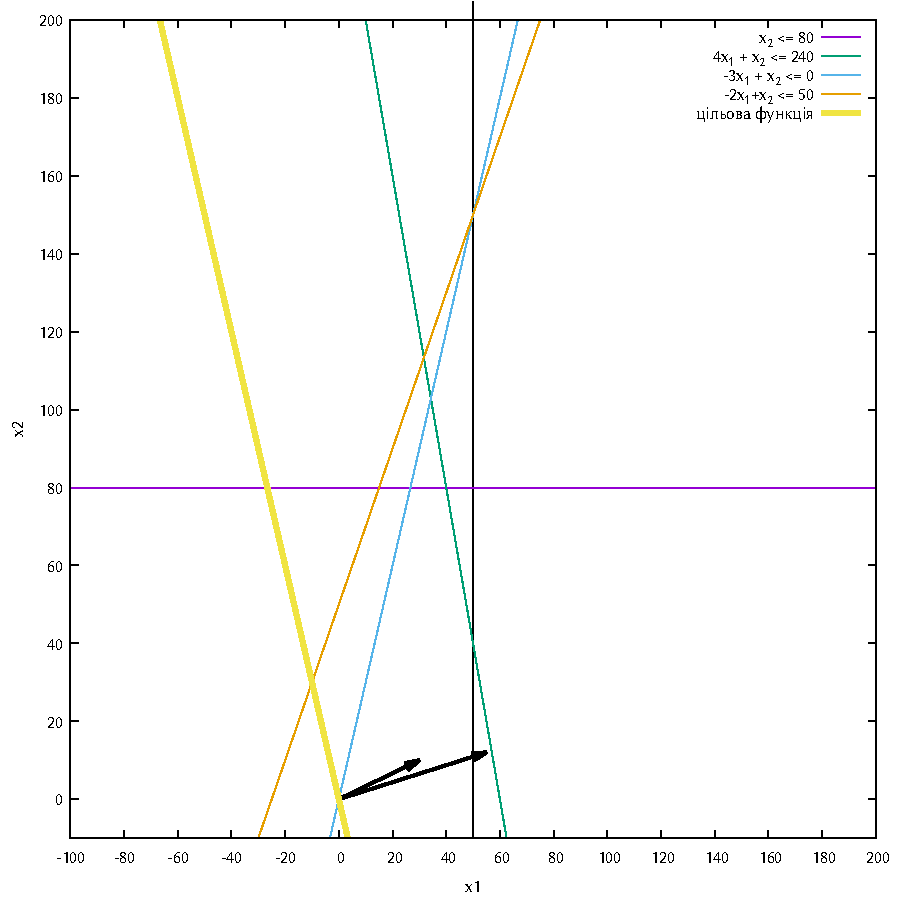
\includegraphics{plot.pdf}
}

\section*{ Висновок}

	\tcobx {
Я написав програму для генерації поліномів лагранжа та
одночасної інтерполяції. З отриманих значень побудував
таблицю та графік за допомогою `gnuplot`. Видно, що
чим більше точок ми використовуємо, тим точніше можемо
відтворити функцію.
}

\end{document}
